% Course adaptation based on IEEEtran bare_conf.tex (Michael Shell).
% IEEEtran.cls and IEEEtran.bst are supplied unchanged under their original licences.
% Main file for Overleaf: main.tex. Compiler: pdfLaTeX (XeLaTeX also supported).
% Replace all instructional prose, sample matrix rows and author placeholders.
\RequirePackage[T1]{fontenc}
\documentclass[conference,a4paper]{IEEEtran}
\usepackage{graphicx}
\usepackage{cite}
\usepackage{array}
\usepackage{url}
\usepackage[hidelinks]{hyperref}
\renewcommand{\dbltopfraction}{0.9}
\setcounter{dbltopnumber}{2}
\hyphenation{in-ter-oper-abil-ity tech-no-log-i-cal}
\begin{document}
\title{
\includegraphics[width=2.8cm]{assets/ulo_estg_logo.png}\\[6pt]
Specific Title of the Review and Project Proposal}
\author{\IEEEauthorblockN{First Author, Second Author, Third Author}
\IEEEauthorblockA{School of Technology and Management, University of Leiria and Oeste, Leiria, Portugal\\
student1@ulo.pt, student2@ulo.pt, student3@ulo.pt\\
Emerging and Intelligent Technologies \textperiodcentered{} Virtual and Augmented Reality \textperiodcentered{} 2026/2027}}
\maketitle
\begin{abstract}
Replace this paragraph with a 150--200-word abstract stating the problem, review scope, literature selection, main findings and implications for the proposed project. Distinguish conclusions supported by the literature from benefits that still need validation. Do not report results for an unimplemented system. Replace all guidance, sample entries and author details before submission. The final paper must contain 6--8 pages including references.
\end{abstract}
\begin{IEEEkeywords}
state of the art; emerging technologies; virtual reality; augmented reality; project proposal
\end{IEEEkeywords}
\section{Introduction}
Introduce the application domain, intended users and problem. Explain its relevance and what existing approaches do not adequately address. Define the review objectives and scope, and explain how the review supports the multidisciplinary project topic approved by the lecturers. Include only the background needed to understand subsequent comparisons and decisions.

Explain how Emerging and Intelligent Technologies (EIT) and Virtual and Augmented Reality (VAR) contribute to the common problem. Justify the use of VR and/or AR for the intended task, considering a conventional alternative where relevant. Define essential terminology and abbreviations.

\subsection{Scope and literature search}
Identify where and when you searched, the main search terms and the criteria used to select material. State practical boundaries such as domain, device type or publication period. A short paragraph is sufficient; formal research questions, a systematic review protocol and a PRISMA diagram are not required. Acknowledge limitations.

\section{State of the Art}
Organise the literature by approaches, themes or comparison criteria. Compare what the studies attempted, the contexts in which they were evaluated, the evidence they produced and the limitations reported. Avoid a sequence of unrelated summaries. Distinguish measured results from authors' expectations, and explain when differences in tasks, datasets, participants or hardware prevent direct comparison.

Use scientific studies for evidence about performance and evaluation, and official documentation for tool capabilities. Foundational literature, such as Azuma's survey \cite{azuma1997}, may provide context; complement it with recent studies relevant to your problem. This example reference does not replace the group's literature selection. IEEE provides the original formatting guidance \cite{ieeeauthor}.

\subsection{Comparative synthesis}
Table~\ref{tab:comparison} illustrates a comparison matrix spanning both columns. Its entries are hypothetical prompts, not published findings. Replace them with evidence from the studies you actually analysed, identifying each source. Select criteria that support a decision in your project. In the text, explain the main patterns, disagreements and gaps revealed by the table; a table alone is not a critical synthesis.


% table* spans BOTH columns. Do not remove the asterisk.
% Two-column floats normally appear at the top of a later page.
\begin{table*}[!t]
\caption{Illustrative literature comparison matrix spanning both columns}
\label{tab:comparison}
\centering
\footnotesize
\setlength{\tabcolsep}{4pt}
\renewcommand{\arraystretch}{1.18}
\begin{tabular}{|>{\raggedright\arraybackslash}p{0.13\textwidth}|>{\raggedright\arraybackslash}p{0.19\textwidth}|>{\raggedright\arraybackslash}p{0.21\textwidth}|>{\raggedright\arraybackslash}p{0.18\textwidth}|>{\raggedright\arraybackslash}p{0.19\textwidth}|}
\hline
\textbf{Study / source} & \textbf{Context and approach} & \textbf{Evidence to extract} & \textbf{Limitation to check} & \textbf{Decision informed} \\ \hline
Study A (replace) & AR task guidance & Task time, errors, sample and protocol & Task specificity; device constraints & Interaction and comparison baseline \\ \hline
Study B (replace) & VR training simulation & Performance, usability and transfer measures & Transfer to real tasks; exposure time & Training scenario and validation plan \\ \hline
Study C (replace) & Sensor-backed service & Latency, reliability and test conditions & Network dependence; controlled setting & Processing location and interface design \\ \hline
\end{tabular}
\vspace{3pt}
\parbox{\textwidth}{\footnotesize The rows above are illustrative prompts, not results from real studies. Replace them with analysed sources and verified evidence.}
\end{table*}

% figure* spans BOTH columns; use figure for a single-column illustration.
\begin{figure*}[!t]
\centering
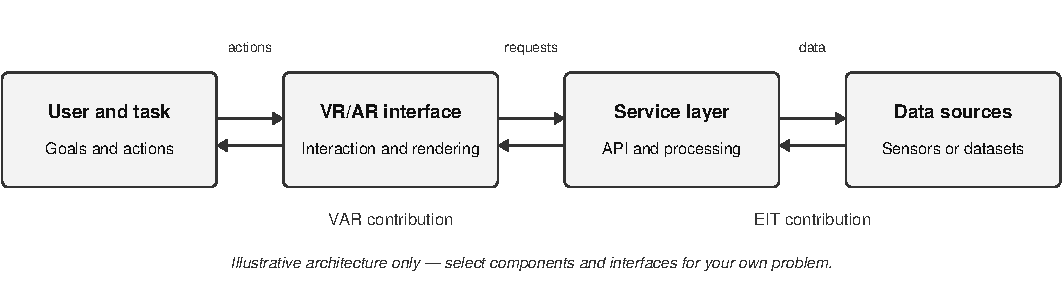
\includegraphics[width=\textwidth]{assets/architecture_example.pdf}
\caption{Illustrative architecture spanning both columns. Arrows represent two-way exchanges; this example does not prescribe a mandatory architecture or report experimental results.}
\label{fig:architecture}
\end{figure*}
\section{Technological Analysis}
Use the reviewed evidence to compare the main technologies, frameworks, devices and architectural approaches being considered. Make the criteria explicit and relate them to the project requirements. Depending on the problem, useful criteria may include interaction capabilities, interoperability, latency, hardware availability, development effort, cost or privacy. Compare credible alternatives and explain which compromises matter most.

Distinguish this section from the State of the Art: that section establishes what existing work demonstrates; this section explains the implications for technological choices. Justify preferred options and identify decisions still open. Product descriptions or popularity alone do not demonstrate suitability.

\section{Project Proposal}
\subsection{Solution and conceptual architecture}
Describe the users, a usage scenario, objectives, essential functionalities and boundaries of the solution. Explain the main components, course-unit contributions and integration interfaces. Fig.~\ref{fig:architecture} illustrates a wide architecture diagram connecting an immersive interface, services and data sources.

Replace the example with your own architecture and labelled data flows. Explain the arrows, where computation occurs and which data are exchanged. Identify equipment, software, data and service dependencies. Include a realistic preliminary development plan and indicate which technology choices remain provisional.

\subsection{Preliminary validation}
Define two or three evaluation criteria or metrics suited to the project. For each, explain what will be assessed, the proposed test, the resources or participants required, and the intended success criterion or how it will be established. Include an appropriate baseline or alternative when useful. Possible choices include task completion time, task errors, usability, interaction accuracy or end-to-end latency; select only those relevant to your objectives.

At this stage, describe how the solution could be validated. An implemented prototype, a completed user study and experimental results are not required. Label expected benefits as hypotheses and identify provisional targets as such. Distinguish the evaluation reported by the reviewed studies from the evaluation planned for your own project.

\section{Discussion}
Discuss the feasibility of the proposal in light of the literature, available resources and semester constraints. Explain the expected technical challenges, integration risks and limitations of the evidence. Consider user comfort, accessibility, privacy or other concerns where they arise from the proposed use. Identify the expected contribution and the assumptions that still need to be tested.

Explain how the review strengthened or changed the proposal, which alternatives were rejected and when decisions might need revision. A justified application, adaptation, integration or evaluation of existing technologies can provide a contribution; distinguish it from unproven novelty.

\section{Conclusions}
Summarise the review findings, resulting decisions and expected contribution. Return to the initial objectives and identify the next development and validation steps. Do not introduce new evidence or claim results that have not been obtained.

\section*{AI Use Declaration}
Replace this guidance with a truthful declaration placed before the references. Identify the tools used, their purpose and the parts of the work they supported. Example with AI: ``The authors used [tool and version] for [purpose] in [sections or tasks]. All outputs were reviewed, and references and technical claims were checked against their sources. The authors remain responsible for the submitted work.'' If no AI was used, state: ``No AI tools were used in the preparation of this work.'' Keep only the declaration that applies.

% Bibliography heading is generated by IEEEtran.
\bibliographystyle{IEEEtran}
\bibliography{references}
\end{document}
